\section{Motivation and Technical Challenges}

Making optimal decisions in real-time is a cornerstone of modern engineering. The necessity of tightly coupling \textbf{discrete decisions} with \textbf{continuous control} is vividly illustrated in advanced robotics:

\begin{itemize}
    \item \textbf{Humanoid Robots (e.g., Boston Dynamics' Atlas):} Navigating complex terrain, such as a parkour course, requires the robot to simultaneously select footstep locations (discrete) and compute the trajectories for its center of mass and limbs (continuous). Currently, solutions often rely on ``hand-coding'' the discrete components, which severely limits the robot's autonomy in novel environments \cite{bostondynamics2021}.
    
    \item \textbf{Industrial Manipulators (e.g., Amazon's Robin):} Sorting efficiency depends on jointly optimizing the sequence of bins (discrete) and the arm's trajectory (continuous) \cite{amazonrobotics2023}. A mere \textbf{1\% increase} in operating speed through superior optimization translates to millions of additional packages processed annually.
\end{itemize}
 
%  2 cols image
\begin{figure}[h]
    \centering
    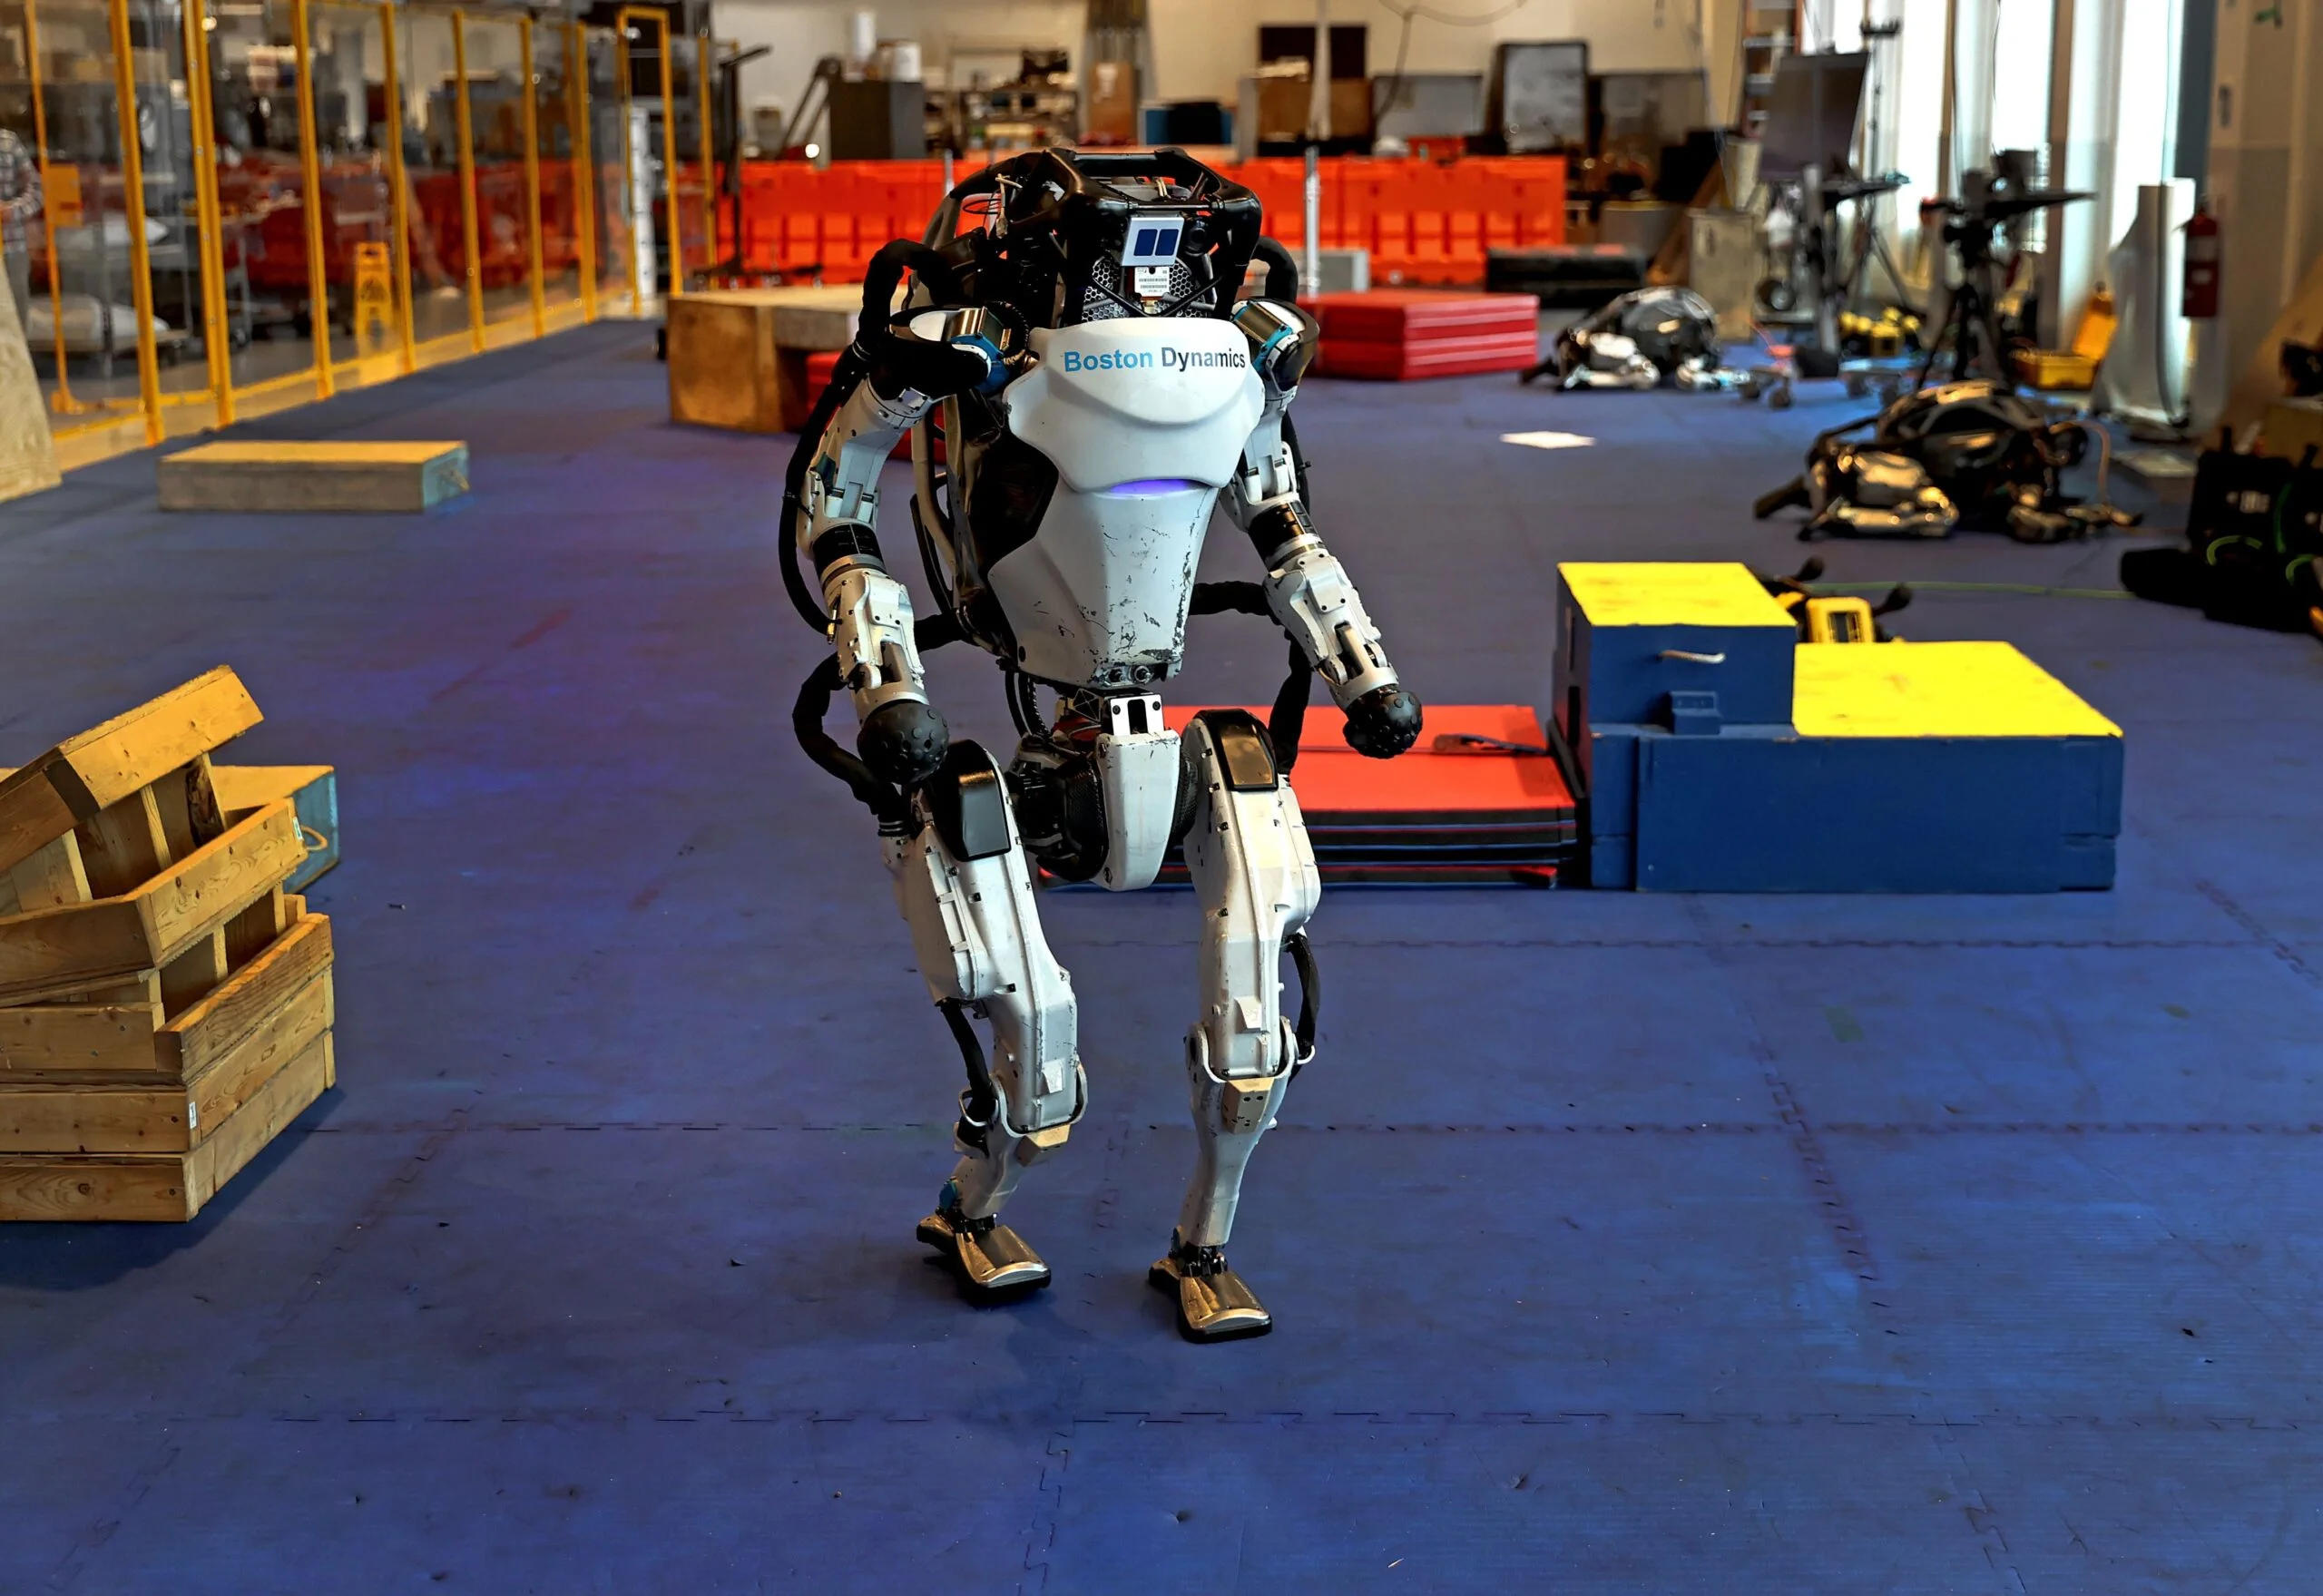
\includegraphics[width=0.475\textwidth]{introduction/image/atlas-robot.png}
    % \hfill
    \includegraphics[width=0.5\textwidth]{introduction/image/aws-robin.png}
    \caption[Boston Dynamics' Atlas and Amazon's Robin]{\textsl{\textbf{Left:} Boston Dynamics' Atlas robot performing parkour, requiring discrete footstep planning and continuous trajectory optimization. \textbf{Right:} Amazon's Robin robotic arm sorting packages, where discrete bin selection and continuous arm trajectory must be optimized jointly.}}
    \label{fig:robotics_examples}
\end{figure}

\hspace{2cm}

However, solving these coupled problems simultaneously remains an open challenge, typically necessitating manual engineering interventions or settling for suboptimal solutions.

Algorithmically, selecting a motion planning method currently forces researchers to compromise between conflicting features: dimensionality, dynamic constraints, and completeness.

\begin{itemize}
    \item \textbf{Trajectory Optimization:} These methods excel at handling robot dynamics and high-dimensional spaces. However, when facing obstacle-cluttered environments—which render the problem inherently nonconvex—they often get trapped in \textbf{local minima}, failing to identify a collision-free trajectory.\cite{diehl2006}
    
    \item \textbf{Sampling-based Planners:} To overcome these limitations, the robotics community frequently resorts to sampling-based methods (e.g., RRT, PRM) due to their ``probabilistic completeness''. However, this comes at a cost: the resulting trajectories are often significantly \textbf{suboptimal}, and imposing \textbf{continuous differential constraints} on discrete samples remains notoriously difficult.\cite{lavalle1998,kavraki1996}
\end{itemize}

\textbf{Mixed-Integer Convex Programming (MICP)} has emerged as a promising solution that bridges this gap. It combines the strengths of both worlds: the completeness of sampling-based algorithms and the dynamic handling capabilities of trajectory optimization, while guaranteeing \textbf{global optimality} within a unified framework. Nevertheless, the adoption of MICP is severely limited by its prohibitive computational costs, often requiring minutes to solve even small-scale problems.

The objective of this research is to break this computational barrier. We focus on a crucial class of motion planning problems involving differential constraints and propose an MICP-based planner capable of reliably solving high-dimensional problems in a matter of seconds through a \textbf{Single Convex Program}.

% \section{Động lực và thách thức kỹ thuật}
